\chapter{Logistic Model}
This chapter focuses on different forms of logistic equation and discuss its properties. In particular, so called \textbf{critical points} are subject of great interest.
In differential equation in the form:

\begin{equation}\label{eq: general form}
du/dt = f(u)
\end{equation}
The roots of this equations are called \textbf{critical points} and have great impact on equation stability.
\section{Malthus Model}
One of the most basic equation describing is an exponential growth equation\footnote{[1]Boyce, Di Prima,\textit{Elementary Differential Equations}; 2013}:
\begin{equation} 
 du/dt = ru
\end{equation}
It first appeared in papers of British mathematician Thomas Malthus in 1798. A constant \textit{r} is called \textbf{rate of growth (if positive) or decline (negative)}. Solving Malthus equation is trivial; with initial condition\footnote{[2] Równania Różniczkowe Zwyczajne, Palczewski A.; 2004}
\begin{equation}
u(0) = u_0
\end{equation}
we have:
\begin{equation}
u = u_0 e^{rt}
\end{equation}
Malthus model can be used to model some populations in a certain, short period of time. However, it is clear, that in the long run, \textit{y(t)} function goes to infinity, which is unrealistic.

\section{Verhulst Model}
Modifying exponential growth, by replacing constant \textit{r} with a function \textit{f(y)}, we obtain:
\begin{equation}
du/dt = f(u)u
\end{equation}
Here, \textit{f(y)} is some function proportional to \textit{r} for small values of \textit{y}, but decreases as \textit{y} grows. The simplest choice is \textit{f(y) = a - by}:

\begin{equation}
du/dt = (a - bu)u
\end{equation}
Where $a$ is a population growth rate, $b > 0$ - self-regulatory effect of crowding on the population an $u$ is
density of population). It is also known as a \textbf{Verhulst equation} or \textbf{logistic equation}\footnote{[1]}. To solve this, we can use separable variables method, that is:
\begin{equation}
\frac{du}{u(1 - \frac{bu}{a})} = adt
\end{equation}
After integrating and setting initial condition $u(0) = u_0$, the solution is following:
\begin{equation}
u = \frac{au_0e^{at}}{bu_0(e^{at}-1) + a}
\end{equation}
If $a > 0$ and $u_0 > 0$ then $u \rightarrow \frac{a}{b}$ for $t \rightarrow \infty$; on the other hand, with $a <0$ and $u_0 > 0$, $u \rightarrow 0$ - those are our two critical points. For convenience, quantity $a/b$ is called $K$

It is convenient to rewrite equation in the form:
\begin{equation} \label{eq:logistic growth}
dy/dt = ry(1 - \frac{y}{K})
\end{equation}

Where \textit{K = r/a}. It is easy to see, that critical points of \ref{eq:logistic growth} are \textit{y = 0} and \textit{y = K}. 

\begin{equation}
\frac{dy}{y(1 - \frac{y}{K})} = rdt
\end{equation}

\begin{equation} \label{eq:logistic growth solution}
y(t) = \frac{y_0 K}{y_0 + e^{-rt}(K - y_0)}
\end{equation}

\begin{figure}[h]
\centering
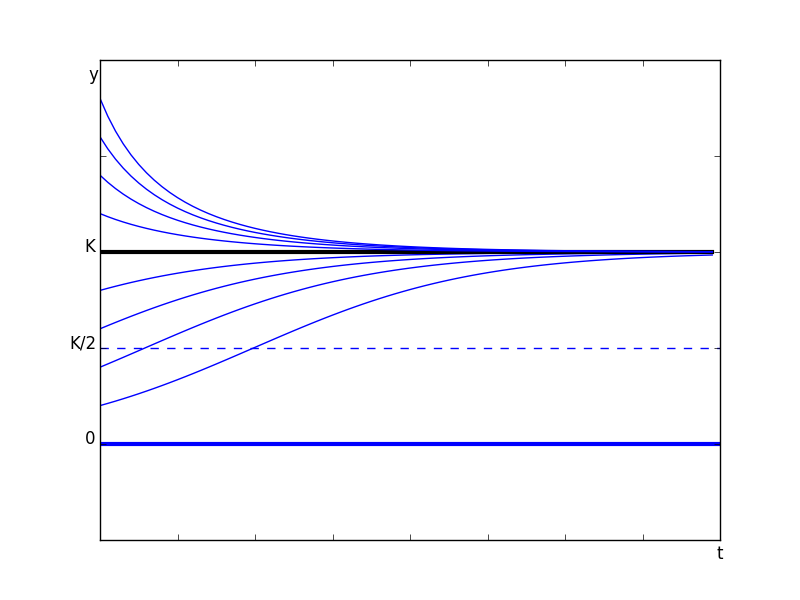
\includegraphics[scale=0.75]{logistic_growth}
\caption{Logistic growth}
\label{fig:logistic growth}
\end{figure}


Looking at graph of few solutions of \ref{eq:logistic growth}, it is clear, that both points $y = 0$ and $y = K$, are critical points of our problem. Indeed, if we substitute $y_0 = 0$, we obtain trivial case when $y(t) = 0$ and for $y0 = K$, from \ref{eq:logistic growth solution}: $y(t) = \frac{K K}{K + (K-K)e^{-rt}} = K$.

In the first case, we say that the solution is \textbf{asymptotically unstable equilibrium}, as for even a small difference from zero, the solution diverges from the given point as $t \rightarrow \infty$. On the other hand, $y(t) = K$ is \textbf{asymptotically stable}, because choosing $y_0$ at any point greater than 0, the solution converges to value K, as $t \rightarrow \infty$.

The value $K$ is called \textbf{limiting population} or \textbf{carrying capacity}\footnote{[3] Elementary Differential Equations, C. Henry Edwards, David E. Penney; 2007}.

\subsection{Critical Threshold}
A small modification (multiplying by -1) to \ref{eq:logistic growth} leads to a similar equation with opposite solution:

\begin{equation} \label{eq:critical treshold}
dy/dt = -ry(1 - \frac{y}{T})
\end{equation}
Again, by separating variables ans substituting $y(0) = y_0$, we obtain:

\begin{equation} \label{eq:critical treshold solution}
y(t) = \frac{y_0 T}{y_0 + e^{-rt}(T - y_0)}
\end{equation}
Parameter $K$ has been changed to $T$ to emphasise, the meaning of the variable, namely \textbf{treshold level}, indicating, that if we start below $T$, the population is going to extinction, which is here indicated as a \textbf{stable} solution. For example, population of mammals needs at least few individual of both sexes to spread out.

\begin{figure}[h]
\centering
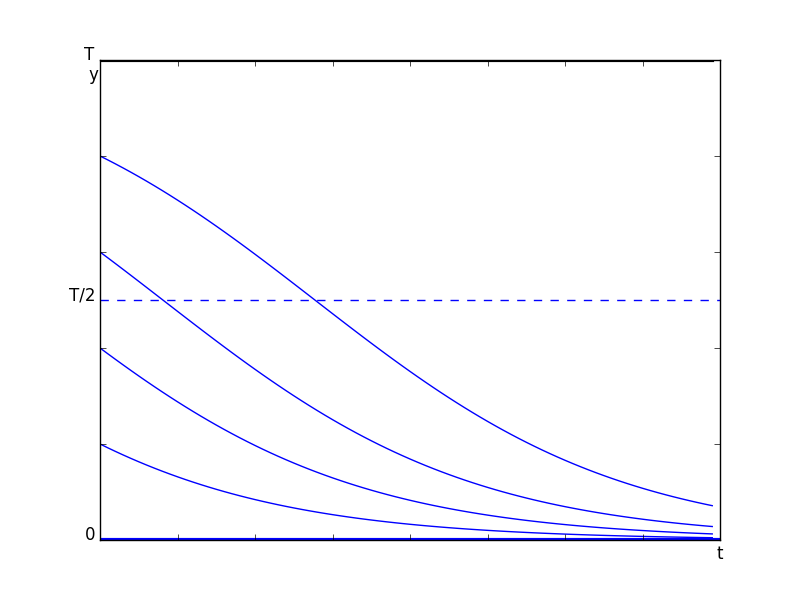
\includegraphics[scale=0.7]{critical_threshold}
\caption{Logistic growth}
\label{fig:logistic growth}
\end{figure}

For an initial populations starting at $y_0 > T$, population growths rapidly, as denominator is going close to zero. At some point on t axis (denoted here as $t_a$) model has a vertical asymptote. It is easy to find this point:
\begin{equation}
y_0 - e^{rt_a}(y_0 - T) = 0 \rightarrow t_a = \frac{1}{r}ln\frac{y_0}{y_0 - T}
\end{equation}

As we can see, this model is a bit more realistic than casual logistic model - it describes the fact, that if too few individuals are present, or available resources (food, space, etc.) are very limited, then population is going to extinction. However, if we above threshold level (exact threshold is unstable solution), then population becomes unbounded, which is unrealistic, so some modification has to be made.

\subsection{Combining logistic model with a threshold}
The most obvious way to solve the problem from the previous paragraph is to combine two models, that is to describe population, that becomes extinct if started below some threshold level (due to lack of minimal amount of individuals or resources), growths above, but eventually stop at some point (indicating for example environment capacity). Such model is described by equation\footnote{[1]}:
\begin{equation} \label{eq: logistic model with a threshold}
dy/dt = -ry(1 - \frac{y}{T})(1 - \frac{y}{K})
\end{equation}

\begin{figure}[h]
\centering
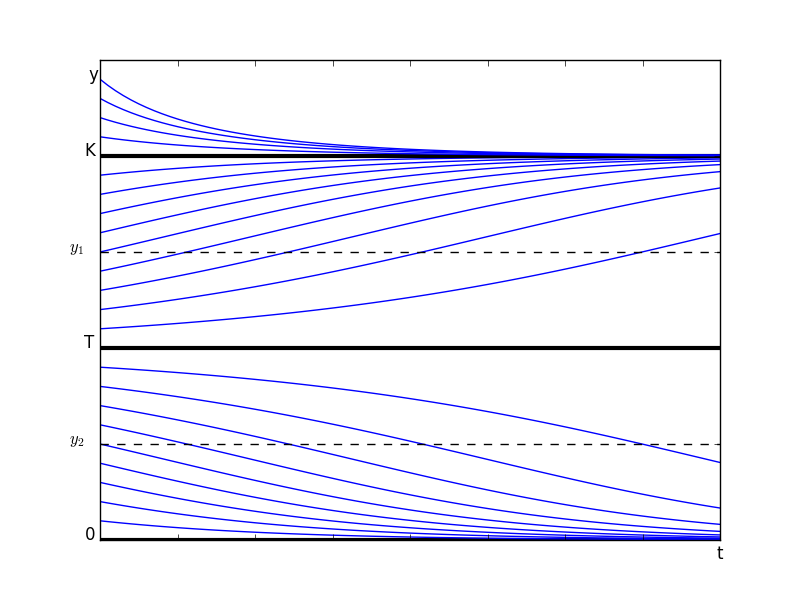
\includegraphics[scale=0.7]{logistic_growth_with_threshold}
\caption{Logistic growth with threshold}
\label{fig:logistic growth}
\end{figure}
As mentioned before, roots of differential equation are stability points. In \ref{eq: logistic model with a threshold} there are 3 roots: $y = 0, y = T, y = K$. First is trivial case, second is the threshold level, below which population extinct, and above with is converging to saturation level $K$ (stable solution) as $t \rightarrow \infty$. In addition, points $y_1$ and $y_2$ denote level at which solution curve changes from concave down to concave up (below $T$) or in opposite way (above $T$).

\section{Bifurcation points}
To generalize the analysis we can observe that \ref{eq: general form} is an equation of variable $y$ and some parameter $\mu$, so we can write this as:

\begin{equation} \label{eq: bifrucation eq}
dy/dt = f(y; \mu)
\end{equation}
\textbf{Bifurcation} of this equation, we call each qualitative change of phase portrait of the equation, that occurs at some point $\mu_0$ - \textbf{bifurcation point}\footnote{[2]}.

Recalling \ref{eq:logistic growth}, we can say this this is equation of the form:

\begin{equation} \label{eq: square bifrucation}
dy/dt = y(a - y)
\end{equation}
We want to determine how equation changes with parameter $a$; we need to break into three different possibilities.

First, when $a = 0$, equation becomes $dy/dt = -y^2$. We could solve it, but at this point it is better to analyse right hand side of the equation, to say how the solution behave. From figure \ref{fig: -yy}, we conclude that solution starting from large values of $y_0$ are approaching level $0$ (our curve is below zero, which means solution decreases); on the other hand, solution starting below this point diverges from zero at large values of $t$ (fro the same reason). Therefore, we say that critical point $0$ is \textbf{semistable} equilibrium, as solutions approach it only from one "side".

\begin{figure}[h]
\centering
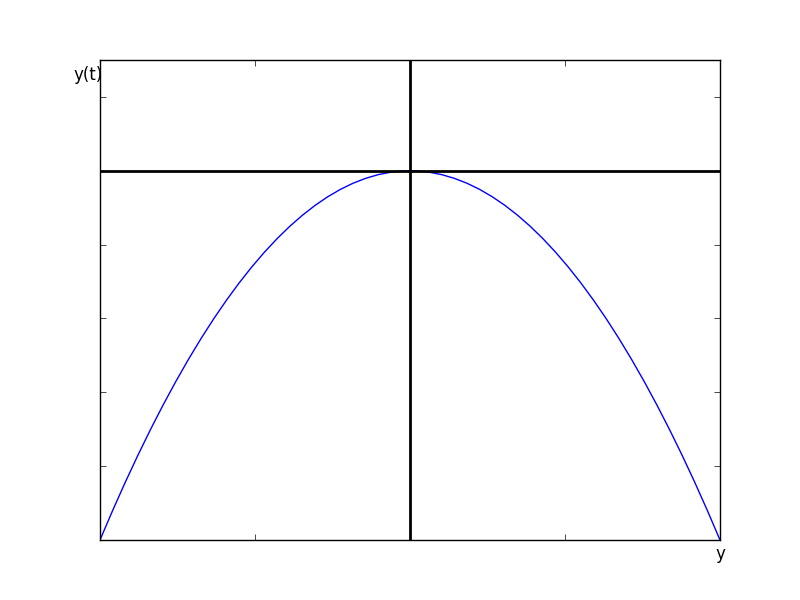
\includegraphics[scale=0.5]{chapter02_yy}
\caption{f(y) versus y for $dy/dt = -y^2$}
\label{fig: -yy}
\end{figure}

\clearpage
Second, when $a < 0$, equation has two critical points-  at $y = 0$ and $y = -a$. This time, solutions starting from infinity towards $-a$ are decreasing, while from $-a$ to $0$ - increasing. From that,we conclude that $y = -a$ is unstable critical point. On the other hand, solutions starting above $y = 0$ decreases with time, converging to $0$, so this point is a stable solution.

\begin{figure}[h]
\centering
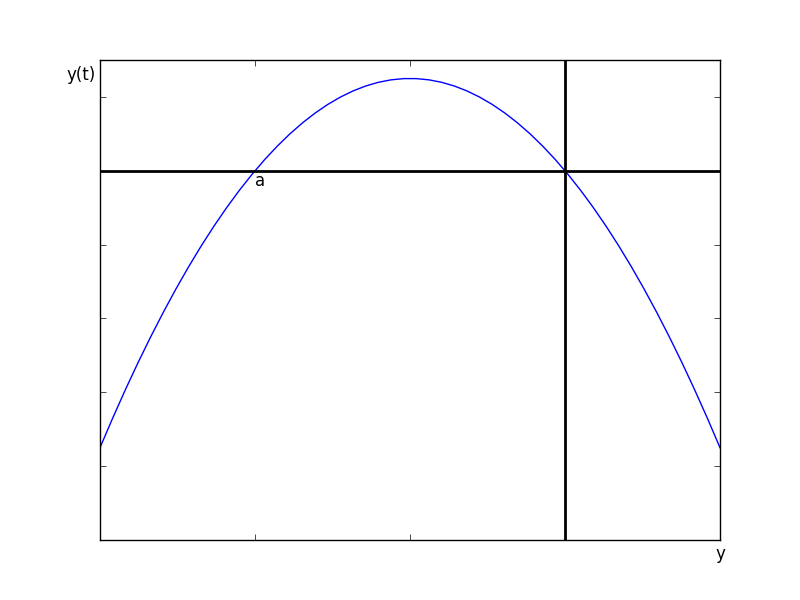
\includegraphics[scale=0.5]{chapter02_y(-1-y)}
\caption{f(y) versus y for $dy/dt = y(a - y)$ for $a < 0$}
\label{fig: y(-a-y)}
\end{figure}

Finally, choosing $a > 0$, we have symmetric to the previous one situation - $y = 0$ is unstable equilibrium, while $y = a$ stable.
\begin{figure}[h]
\centering
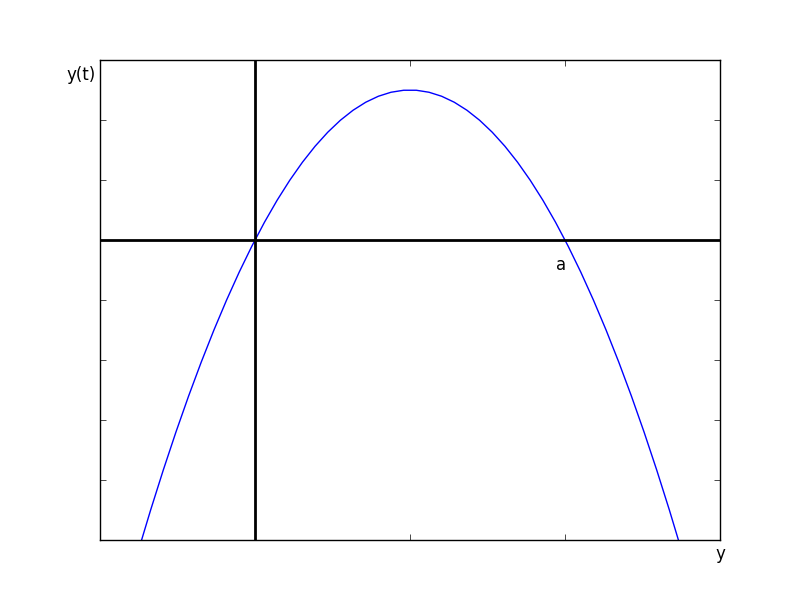
\includegraphics[scale=0.5]{chapter02_y(1-y)}
\caption{f(y) versus y for $dy/dt = y(a - y)$ for $a > 0$}
\label{fig: y(a-y)}
\end{figure}

\subsection{Bifurcation diagrams}
A common way to illustrate how stability changes with different parameters $a$ is to plot \textbf{bifurcation diagram} - graph with values of $a$ in the horizontal axis and critical points (denoted here as $c$) on vertical axis. Dash line represents unstable, while solid line stable equilibria.

\begin{figure}[h]
\centering
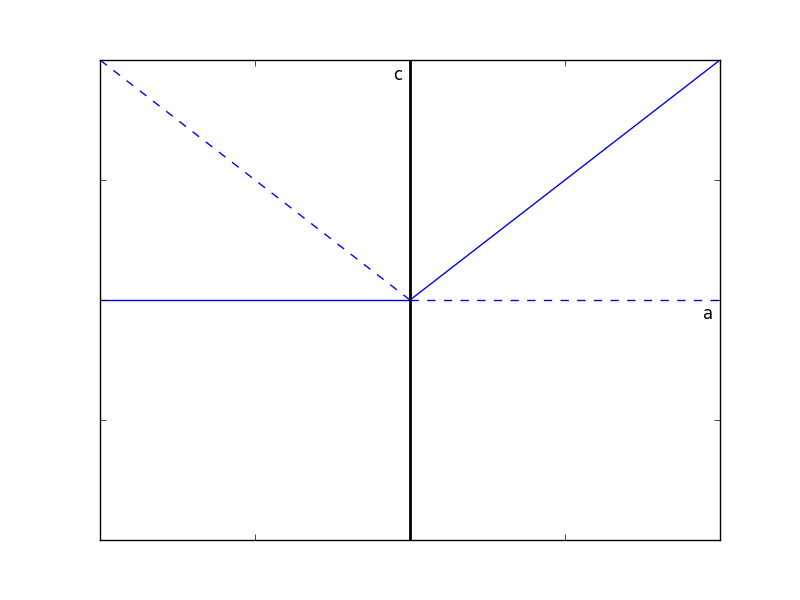
\includegraphics[scale=0.5]{chapter02_bifr_y(a-y)}
\caption{Bifurcation diagram for different values of $a$ in $dy/dt = y(a-y)$}
\label{fig: bifr_y(a-y)}
\end{figure}
Such behaviour is called \textbf{transcritical bifurcation}\footnote{[1]}, as in some point (here $a = 0$) we observe exchange of stability, as solutions that was unstable before reaching this value, becomes stable.

Similar analysis can be done for equation \ref{eq: logistic model with a threshold}. For simplicity, assuming $T = K$, we obtain equation in the form:

\begin{equation}\label{eq: bifr_y(a-yy)}
dy/dt = y(\sqrt{a}-y)(\sqrt{a}+y) = y(a - y^2)
\end{equation}
For $a = 0$ and $a < 0$ we have one stable critical point at $y = 0$. For $a > 0$ solution has two stable equilibria at $y = +/- \sqrt{a}$ and one unstable at $y = 0$. This kind of bifurcation is knows as \textbf{pitchfork bifurcation}\footnote{[3]}.

\begin{figure}[h]
\centering
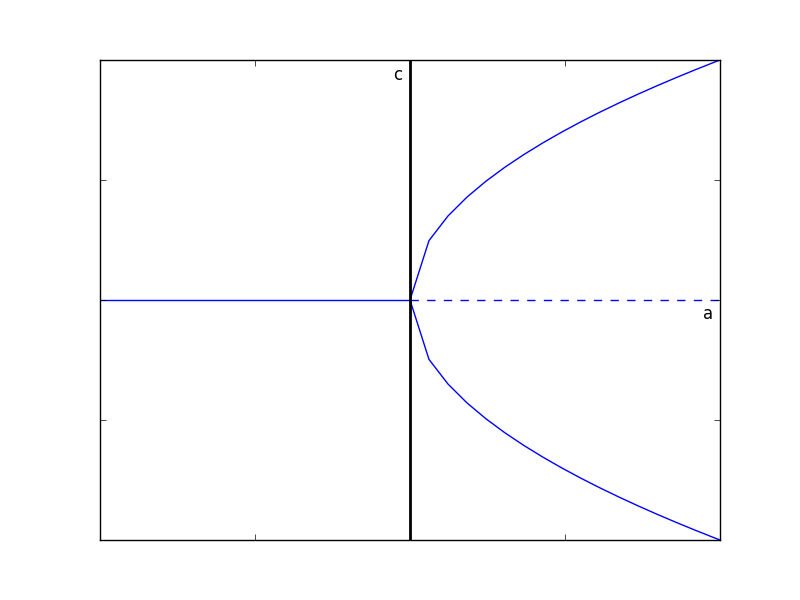
\includegraphics[scale=0.5]{chapter02_bifr_pitch}
\caption{Bifurcation diagram for different values of $a$ in $dy/dt = y(a-y^2)$}
\label{fig: bifr_pitch}
\end{figure}